\documentclass[11pt]{article}
\usepackage[utf8]{inputenc}	% Para caracteres en español
\usepackage{amsmath,amsthm,amsfonts,amssymb,amscd}
\usepackage{multirow,booktabs}
\usepackage[table]{xcolor}
\usepackage{fullpage}
\usepackage{lastpage}
\usepackage{enumitem}
\usepackage{fancyhdr}
\usepackage{mathrsfs}
\usepackage{wrapfig}
\usepackage{setspace}
\usepackage{calc}
\usepackage{multicol}
\usepackage{cancel}
\usepackage[retainorgcmds]{IEEEtrantools}
\usepackage[margin=3cm]{geometry}
\usepackage{amsmath}
\newlength{\tabcont}
\setlength{\parindent}{0.0in}
\setlength{\parskip}{0.05in}
\usepackage{empheq}
\usepackage{framed}
\usepackage[most]{tcolorbox}
\usepackage{xcolor}
\colorlet{shadecolor}{orange!15}
\parindent 0in
\parskip 12pt
\geometry{margin=1in, headsep=0.25in}
\theoremstyle{definition}
\newtheorem{defn}{Definition}
\newtheorem{reg}{Rule}
\newtheorem{exer}{Exercise}
\newtheorem{sln}{Solution}
\newtheorem{note}{Note}
\begin{document}
\setcounter{section}{0}
\title{Math lecs 15,16,17 review}

\thispagestyle{empty}
\tableofcontents
\begin{center}
{\LARGE \bf Lectures 18,19,20}\\
{\large \bf Math301}\\
Fall 2020
\end{center}

\section{Power Series REV}
it's a series of the form \\
\[ \sum_{n=0}^{\infty} c_n(x-a)^n = c_0 + c_1(x-a) + c_2(x-a)^2 + c_3(x-a)^3 + ...  \]
\\
it's called a power series about $x=a$
\begin{enumerate}

\item The series converges only when x =a 
\item the series converges for all x
\item convergent on an interval called interval of convergence such that it's convergent when  $ |x-a| < R $ and divergent when $|x-a|>R$

\subsection{How to get R}
$R$ or the \textbf{radius of convergence} can be calculated using the following formulas: \\
\begin{align}
	R = \frac{1}{\lim_{n \to \infty} \frac{c_{n+1}}{c_n}} && \text{or} &&  R = \frac{1}{\lim_{n \to \infty} \sqrt{|c_n|}}
\end{align}

\end{enumerate}
\subsection{Interval of convergence}
the power series is said to be convergent on the following  interval :
$ [-R+a , R+a ]  $ and the interval can either be closed or open in any ending so we have to test all the sitiuations
\begin{reg}
	if \[ f(x) =  \sum_{n=0}^{\infty} c_n(x-a)^n \] 
	then   $c_n = \frac{f^{(n)} (a)}{n!} $ 
\end{reg}
so; 
\begin{enumerate}

\item if $\sum = 0 \to c_n = 0 $ 
\item if $ \sum a_n(x-a)^n = \sum b_n(x-1)^n \to a_n = b_n $ 

\end{enumerate}
\subsection{Term by term summation}
\begin{equation}
	\sum_{n=0}^{\infty} a_n (x-a)^n + \sum_{n=0}^{\infty} b_n(x-1)^n = \sum_{n=0}^{\infty} [a_n+b_n] (x-a)^n
\end{equation}
this is applicable if \begin{enumerate}

\item the two $\sum$s start and end with the same values

\end{enumerate}
\subsection{term by term differentiation}
this is basically: the derivative on the $\sum$s is the $\sum$ of the derivatives  
\begin{note}
	The Radii of convergence of both $f(x), f'(x)$ are the same 
\end{note}
\subsection{series expansions of basic functions}
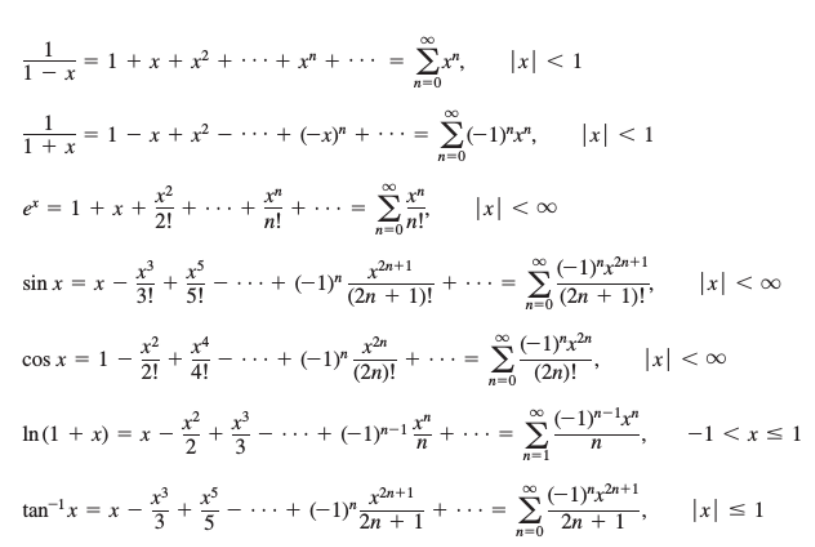
\includegraphics[scale=0.5]{images/img1.png}
\subsection{Re-indexing sums}
if you drop down in on side you rise up in the other one 
\begin{equation}
\sum_{n=k}^{\infty} a_n = \sum_{n=0}^{\infty} a_{n+k} 
\end{equation}
\begin{equation}
\sum_{n=k}^{\infty} a_n = \sum_{n=k+h}^{\infty} a_{n-h} 
\end{equation}

\section{Solving ODEs using power series method}
the method is so simple, you assume that $y = \sum_{n=0}^{\infty} a_nx^n$ and this leads to having $y' = \sum_{n=1}^{\infty} na_nx^{n-1}$ and $y'' = \sum_{n=2}^{\infty} n(n-1)a_nx^{n-2}$ \textbf{note the n in all sums}
\\ and then we solve them together. to solve and sum them; they all must have the same n and all $X$s must have the same power. In order to achieve that do the following :
\begin{enumerate}

\item try to change powers of x in all sums to be the same
\item then change the n of them by either method of the following
	\begin{enumerate}
	
	\item re-indexing
	\item expanding some terms of the series
	
	\end{enumerate}

\end{enumerate}
all we want to have to solve the ODE is the $a_n$ (the coeffiecients in the series) and we can get them by substitution. Of course we can't get theme explicitly. You will eventually get a recurrence relation to solve. it can be solved either by substuting in it multiple times to have the final coeffiecients or by notice. 
\begin{equation}
	C_{n+2} = - \frac{(2n-1)}{(n+2)(n+1)} C_n \to  n = 0,1,2,3,4,...
\end{equation}
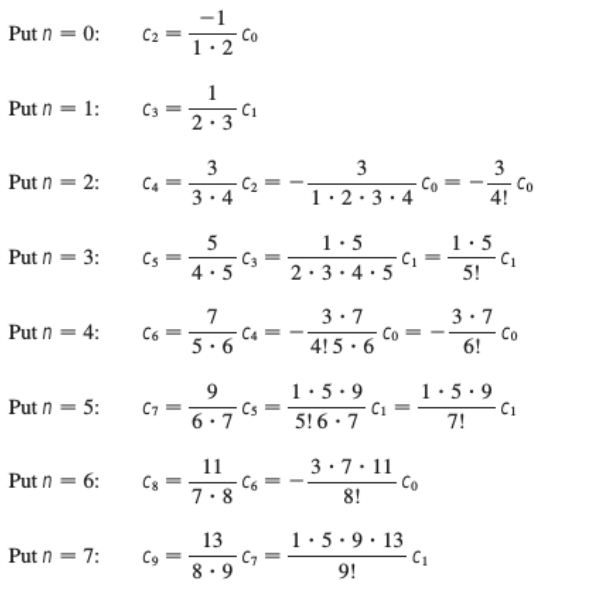
\includegraphics[scale=0.5]{images/img2.png}
\\
the pattern can be detected, as we have two patterns one for the even part and one for the odd
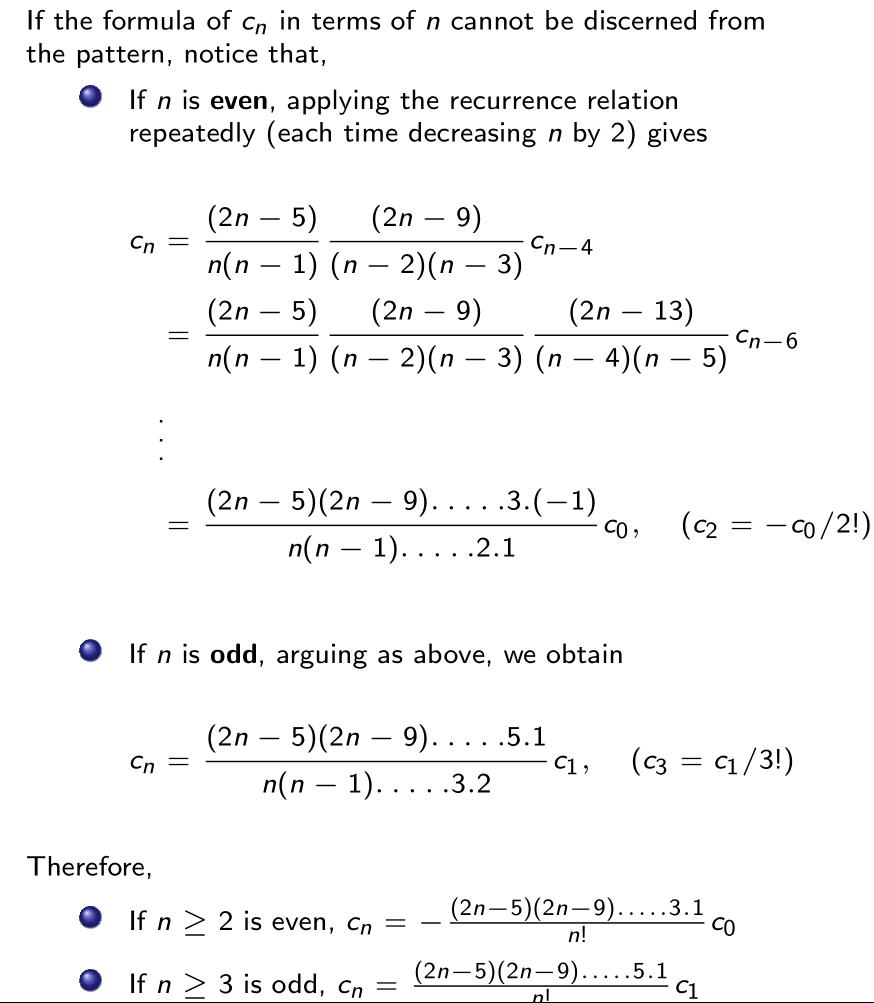
\includegraphics[scale=0.5]{images/img3.png}

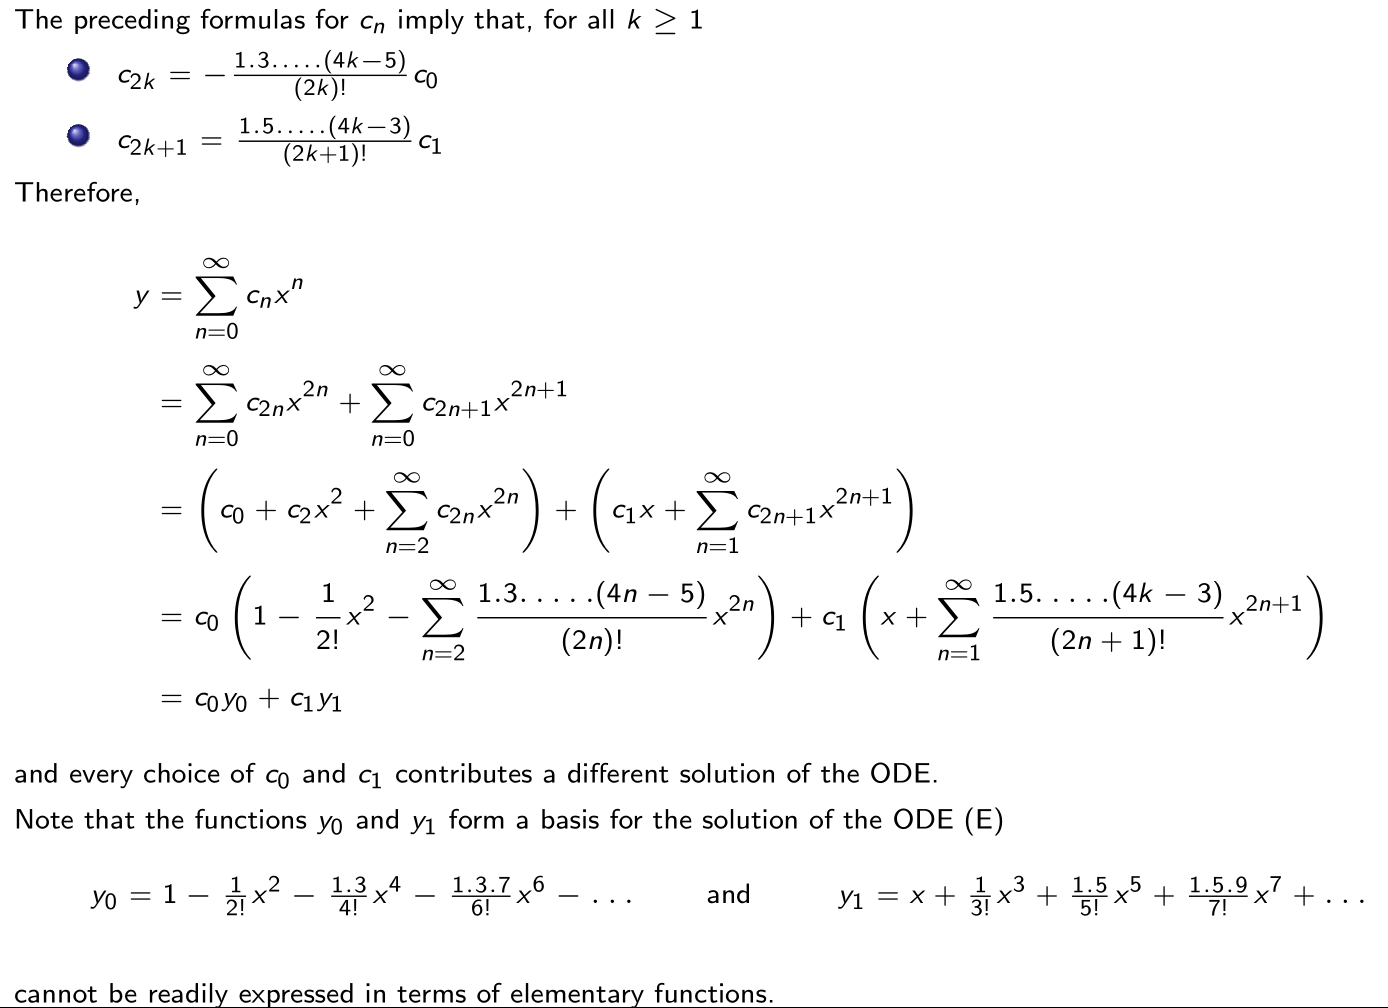
\includegraphics[scale=0.5]{images/img4.png}
\begin{note}
Sometimes the functions $y_1,y_2$ can be basic functions so you have to recall the power series expansions of them to have the solution in the standard form.
\end{note}
\begin{note}
in the last example we expanded the series because we can't substitute in the value of the coeffiecients unless the series starts from n=1 or n= any number that is indicated above in the question.
\end{note}
\begin{exer}
Solve the Following ODE using power series method. 
\begin{equation}
y' - x^2y = 0
\end{equation}
\end{exer}
\begin{sln}

\begin{align}
	let\\ y = \sum_{n=0}^{\infty}a_n x^n && y' = \sum_{n=1}^{\infty} na_nx^{n-1} \\
	\sum_{n=1}^{\infty} na_nx^{n-1} - x^2 (\sum_{n=0}^{\infty}) = 0\\
\end{align}

\end{sln}

\end{document}

